\documentclass[11pt]{article}

\usepackage[utf8]{inputenc}
\usepackage[T1]{fontenc}
\usepackage{lmodern}
\usepackage{amsmath,amssymb}
\usepackage[numbers,round]{natbib}
\usepackage{booktabs}
\usepackage{graphicx}
\usepackage{geometry}
\usepackage[expansion=false]{microtype}
\usepackage[hidelinks]{hyperref}
\usepackage{setspace}
\usepackage{lineno}
\geometry{letterpaper,margin=1in}
\doublespacing
\linenumbers

\newcommand{\demodex}{\textit{Demodex}}

\title{\textit{Fusobacterium} depletion is a reproducible bacterial correlate of
ocular \demodex{} disease: a three-cohort meta-analysis across 16S amplicon and
shotgun sequencing}
\author{Jonathan Reich \\
  {\small Independent Researcher, Melbourne, Victoria, Australia} \\
  {\small Corresponding author: \texttt{jonathanreich100@gmail.com}} \\
  {\small ORCID: \href{https://orcid.org/0009-0000-0108-0717}{0009-0000-0108-0717}}}
\date{}

\begin{document}
\maketitle

\begin{abstract}
\textbf{Background.} Infestation of the ocular surface and eyelids by \demodex{}
mites drives blepharitis and is tightly linked to rosacea, but the accompanying
bacterial community is contested: individual surveys have variously implicated
\textit{Pseudomonas}, \textit{Acinetobacter}, \textit{Cutibacterium},
\textit{Streptococcus} and \textit{Corynebacterium}, among others, with little
agreement between studies. Whether
\emph{any} bacterial genus tracks ocular \demodex{} disease reproducibly---across
independent cohorts and across sequencing technologies---is unknown.
\textbf{Methods.} We uniformly reprocessed three independent public ocular-surface
cohorts (111 subjects; 69 \demodex{}, 42 control): two conjunctival 16S amplicon
studies (V4 and V3--V4) denoised to amplicon sequence variants with DADA2 and
classified against SILVA~v138.1, and one conjunctival shotgun-metagenomic study
classified with Kraken2/Bracken. Per cohort we computed genus-level
Mann--Whitney statistics; we then combined them by a sample-size-weighted
Stouffer $Z$ over the 38 genera present in $\ge$50\% of samples in \emph{every}
cohort, with Benjamini--Hochberg control of the false-discovery rate,
leave-one-cohort-out re-analysis, and---for the shotgun cohort---explicit tests
for host-DNA and depth confounding.
\textbf{Results.} A single genus, \textit{Fusobacterium}, was depleted in
\demodex{} disease concordantly in all three cohorts (per-cohort AUC $0.33$,
$0.31$, $0.36$; combined $Z=-2.93$, $p=0.0034$, $q=0.088$). It was the
top-ranked genus overall and the only one that remained significant
($p<0.05$) when any single cohort was removed. In the shotgun cohort the
depletion was independent of host-DNA fraction and sequencing depth (both
$p>0.8$) and held under every normalisation (present in $21/25$ cases vs
$11/11$ controls). \textit{Corynebacterium} was concordantly enriched but weak
($p=0.16$). Genera prominent in single reports---\textit{Neisseria},
\textit{Rothia}, \textit{Streptococcus}---did \emph{not} reproduce, reversing
direction between cohorts.
\textbf{Conclusions.} Across independent cohorts and two sequencing
methodologies, \textit{Fusobacterium} depletion is the leading reproducible
bacterial correlate of ocular \demodex{} disease and a defensible target for
mechanistic and diagnostic follow-up, whereas the field's single-cohort leads
largely do not replicate. No genus survived Bonferroni correction at three
cohorts, a limitation that additional cohorts would resolve.
\end{abstract}

\section*{Importance}
Microbiome case--control studies are famously hard to reproduce: each cohort
tends to nominate its own ``signature'' organisms, and readers cannot tell which
findings are real. \demodex{} mites of the eyelids and ocular surface---close
relatives of the mites that colonise rosacea skin---are a case in point, with
published bacterial associations that scarcely overlap. We take the opposite tack
to a single new survey: we re-analyse three independent public cohorts through one
consistent pipeline and ask which genus-level differences \emph{survive} being
tested in every cohort, including a switch from 16S amplicon to shotgun
metagenomic sequencing. Only one genus does---\textit{Fusobacterium}, consistently
depleted where mites are present---while several widely cited candidates do not
replicate. The result gives the field a concrete, reproducible target instead of a
longer list of cohort-specific names, and illustrates a template for separating
durable microbiome signals from statistical noise.

\section{Introduction}

\demodex{} mites (\textit{D.\ folliculorum} and \textit{D.\ brevis}) colonise the
human pilosebaceous unit and the eyelash follicles and meibomian glands of the
ocular surface. Their density is markedly elevated in rosacea---a meta-analysis of
23 case--control studies placed the odds ratio for infestation near nine
\citep{chang2017}---and \demodex{} infestation is a recognised driver of chronic
blepharitis and ocular-surface inflammation. Because the mite lives in intimate
contact with the resident bacterial community, a natural hypothesis is that
\demodex{} colonisation reshapes the ocular-surface microbiome, and that the shift
might mark, or even mediate, disease.

Testing that hypothesis has produced a fragmented literature. Conjunctival 16S
surveys have variously reported that \textit{Pseudomonas}, \textit{Acinetobacter}
and \textit{Bacillus} dominate the infested ocular surface, with relative
increases in \textit{Acinetobacter} and \textit{Novosphingobium} and decreases in
others \citep{liang2021}; that \textit{Lactobacillus} and \textit{Bifidobacterium}
are enriched with mite carriage \citep{yan2020}; and shotgun metagenomics of
conjunctiva and meibum
has emphasised \textit{Cutibacterium} and \textit{Pseudomonas} changes together
with elevated \textit{Acinetobacter}, \textit{Sphingobium} and \textit{Delftia}
\citep{fu2022}. An eyelash 16S study instead highlighted a depletion of
\textit{Burkholderia} and an enrichment of \textit{Corynebacterium} in \demodex{}
blepharitis \citep{zou2024}. The genus-level ``hits'' differ from study to study,
and no candidate has been shown to reproduce across cohorts, let alone across
sequencing platforms. This is the familiar reproducibility problem of microbiome
case--control work: small cohorts, divergent sampling sites and amplicon regions,
and study-specific contaminants together generate long lists of significant but
non-replicating taxa.

We therefore ask a deliberately conservative, positive question: is there
\emph{any} bacterial genus whose association with ocular \demodex{} disease
reproduces across independent cohorts and across sequencing methodologies? Rather
than analyse one new dataset, we assemble three public ocular-surface cohorts,
reprocess each from raw reads through a single consistent pipeline, and combine
them by formal meta-analysis. We require a genuine signal to be (i) present at
reasonable prevalence in every cohort, (ii) concordant in direction across all of
them, and (iii) robust to removing any one cohort---criteria that suppress the
cohort-specific artefacts that inflate single-study findings. One genus,
\textit{Fusobacterium}, meets all three; several prominent single-cohort
candidates do not.

\section{Materials and methods}

\subsection{Cohorts}
We analysed three independent public studies of the human ocular surface in which
subjects were classified as \demodex{}-infested (cases) or uninfested (controls),
all sampling the conjunctiva/ocular surface (Table~\ref{tab:cohorts}). Two are 16S
rRNA amplicon studies---a discovery cohort sequencing the V4 region
\citep{liang2021} and a replication cohort sequencing V3--V4 \citep{yan2020}---and
one is a shotgun-metagenomic study \citep{fu2022}. Case/control labels were taken
from the studies' own sample metadata (sample aliases and BioSample attributes).
In total 111 subjects were analysed (69 \demodex{}, 42 control). A fourth ocular
\demodex{} 16S cohort (eyelash, V3--V4; \citealp{zou2024}) is discussed for
external corroboration but could not be pooled: its per-sample data are not
publicly available and its repository was not retrievable (see
Sec.~\ref{sec:disc}).

\begin{table}[t]
\centering
\small
\begin{tabular}{lllrr}
\toprule
cohort (label) & accession & platform / target & \demodex{} & control \\
\midrule
discovery \citep{liang2021}   & PRJNA692647 & Illumina, 16S V4 (515F/806R)      & 14 & 17 \\
rep2020 \citep{yan2020}       & PRJNA657256 & Illumina MiSeq, 16S V3--V4 (338F/806R) & 30 & 14 \\
shotgun2022 \citep{fu2022}    & PRJNA856121 & Illumina, shotgun WGS (75\,bp SE) & 25 & 11 \\
\midrule
\multicolumn{3}{l}{\textbf{total}} & \textbf{69} & \textbf{42} \\
\bottomrule
\end{tabular}
\caption{The three independent conjunctival/ocular-surface cohorts, uniformly
reprocessed here. All compare \demodex{}-infested cases with uninfested controls.}
\label{tab:cohorts}
\end{table}

\subsection{16S amplicon processing (discovery, rep2020)}
Paired-end reads were retrieved from the European Nucleotide Archive. Primers were
removed with \texttt{cutadapt} \citep{martin2011} (515F/806R for the V4 discovery
cohort; 338F/806R for the V3--V4 replication cohort), and reads were denoised into
amplicon sequence variants (ASVs) with DADA2 \citep{callahan2016} using
\texttt{filterAndTrim}, \texttt{learnErrors}, \texttt{dada}, \texttt{mergePairs}
and \texttt{removeBimeraDenovo}. Taxonomy was assigned against the SILVA v138.1
training set \citep{quast2013}. ASVs were collapsed to genus for the cross-cohort
analysis. Exact-sequence (ASV) resolution was used rather than closed-reference or
OTU clustering because it avoids the species-level misassignment to which
short-read marker-gene data are otherwise prone \citep{callahan2017}.

\subsection{Shotgun metagenomic classification (shotgun2022)}
Single-end 75\,bp reads were classified with Kraken2 \citep{kraken2} against the
standard database (bacteria, archaea, viral, human, UniVec), and genus-level
abundances were re-estimated with Bracken \citep{bracken} using the 75-mer
distribution matched to the read length. Read counts were restricted to genera
whose NCBI lineage lies within Bacteria, so that host and viral reads are excluded
and abundances are expressed relative to the bacterial community---comparable to
the 16S cohorts. NCBI genus names coincide with SILVA genus names for the taxa of
interest here (e.g.\ \textit{Fusobacterium}, \textit{Corynebacterium},
\textit{Pseudomonas}), enabling a common genus vocabulary across platforms.

\subsection{Cross-cohort meta-analysis}
Within each cohort, every genus was tested for a difference between cases and
controls with the tie-corrected Mann--Whitney $U$ test on genus relative
abundance, yielding a signed standard-normal statistic $z$ (positive $=$ enriched
in \demodex{}) and the rank-biserial ROC-AUC. To suppress study-specific
contaminants---which are typically present in only one cohort---we restricted the
meta-analysis to the 38 genera present (relative abundance $>0$) in at least
50\% of samples in \emph{every} cohort. For each such genus the per-cohort $z$
values were combined into a single Stouffer statistic weighted by $\sqrt{n}$,
$Z=\sum_i \sqrt{n_i}\,z_i \big/ \sqrt{\sum_i n_i}$, whose two-sided $p$-value
follows the standard normal \citep{whitlock2005}. A genus was termed
\emph{concordant} when its per-cohort $z$ shared the same sign in all three
cohorts. Multiple testing over the 38 genera was controlled both by the
conservative Bonferroni bound and by the Benjamini--Hochberg false-discovery rate
($q$-value) \citep{bh1995}.

\subsection{Robustness and confounder analyses}
Two additional analyses guard against a result being driven by one cohort or by a
technical artefact. First, a leave-one-cohort-out analysis recomputed the combined
$Z$ (and $p$) after dropping each cohort in turn; a robust signal keeps its sign
and comparable magnitude throughout. Second, because ocular shotgun samples are
dominated by host DNA, we used the Kraken2 reports to test, for the shotgun
cohort, whether cases and controls differed in total sequencing depth, in host-DNA
fraction (\textit{Homo} reads / total), or in total bacterial reads (Mann--Whitney),
and whether the \textit{Fusobacterium} result persisted under three
normalisations (fraction of bacterial reads, fraction of total reads, and
reads-per-million) and as simple presence/absence. All statistics were computed
with a pure-Python implementation (tie-corrected Mann--Whitney $U$, Stouffer $Z$,
Benjamini--Hochberg, Spearman) released with the code.

\section{Results}

\subsection{One genus, \textit{Fusobacterium}, is depleted in \demodex{} disease
across all three cohorts}
Of the 38 genera present in at least half of the samples of every cohort,
\textit{Fusobacterium} showed the strongest cross-cohort signal: it was depleted
in \demodex{} cases in all three cohorts (per-cohort AUC $0.332$, $0.305$,
$0.360$; all $<0.5$), giving a combined $Z=-2.93$ ($p=0.0034$) and the smallest
false-discovery-rate $q$-value in the analysis ($q=0.088$, tied with
\textit{Bradyrhizobium}; Table~\ref{tab:meta}). The direction was perfectly
concordant, and the effect is visible as three points lying entirely to the
depleted side of chance in Fig.~\ref{fig:auc}. \textit{Corynebacterium} was the
strongest concordant \emph{enrichment} (AUC $0.685$, $0.555$, $0.520$; combined
$Z=+1.40$, $p=0.16$), consistent in direction across cohorts but individually
weak.

\begin{table}[t]
\centering
\small
\begin{tabular}{lcrrrcccc}
\toprule
genus & dir. & $Z$ & $p$ & $q_{\mathrm{BH}}$ & concord. & AUC$_{\mathrm{disc}}$ & AUC$_{\mathrm{rep}}$ & AUC$_{\mathrm{shot}}$ \\
\midrule
\textit{Fusobacterium}   & down & $-2.93$ & 0.0034 & 0.088 & yes & 0.332 & 0.305 & 0.360 \\
\textit{Bradyrhizobium}  & up   & $+2.83$ & 0.0046 & 0.088 & yes$^\dagger$ & 0.668 & 0.520 & 0.844 \\
\textit{Brevundimonas}   & down & $-2.11$ & 0.035  & 0.325 & yes$^\dagger$ & 0.366 & 0.452 & 0.291 \\
\textit{Corynebacterium} & up   & $+1.40$ & 0.163  & 0.402 & yes & 0.685 & 0.555 & 0.520 \\
\textit{Neisseria}       & --   & $-1.79$ & 0.073  & 0.325 & no  & 0.689 & 0.321 & 0.222 \\
\textit{Rothia}          & up   & $+0.94$ & 0.347  & 0.527 & no  & 0.729 & 0.590 & 0.347 \\
\textit{Streptococcus}   & up   & $+0.93$ & 0.352  & 0.527 & no  & 0.664 & 0.617 & 0.376 \\
\bottomrule
\end{tabular}
\caption{Meta-analysis of selected genera across the three cohorts (full ranking
of all 38 genera in the released output). $Z$ and $p$ are the $\sqrt{n}$-weighted
Stouffer statistic and its two-sided $p$-value; $q_{\mathrm{BH}}$ is the
Benjamini--Hochberg false-discovery rate over 38 genera; ``concord.'' marks genera
with the same direction in all three cohorts. AUC columns are the per-cohort
Demodex$>$control ROC-AUC (values $<0.5$ indicate depletion). $^\dagger$Concordant
but not robust to leave-one-cohort-out (Table~\ref{tab:loo}); both are common
environmental/reagent genera.}
\label{tab:meta}
\end{table}

\begin{figure}[t]
\centering
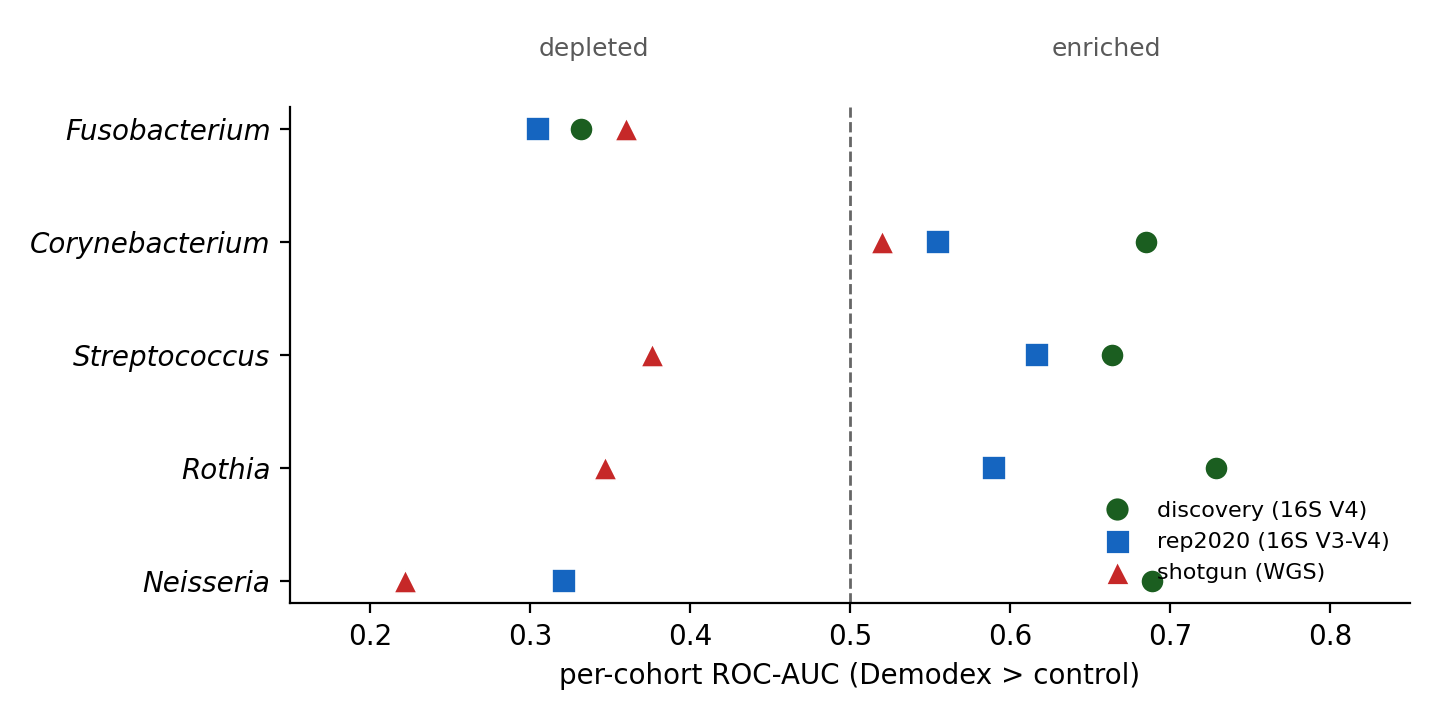
\includegraphics[width=0.82\textwidth]{results/fig_meta_auc.png}
\caption{Per-cohort ROC-AUC (Demodex$>$control) for reproducible versus
non-reproducible genera. Each genus has one point per cohort (discovery, 16S V4;
rep2020, 16S V3--V4; shotgun, WGS); the dashed line is chance (AUC $0.5$).
\textit{Fusobacterium} lies entirely on the depleted side and
\textit{Corynebacterium} entirely on the enriched side in all three cohorts,
whereas \textit{Streptococcus}, \textit{Rothia} and \textit{Neisseria}---each
prominent in an individual study---straddle chance and therefore do not reproduce.}
\label{fig:auc}
\end{figure}

\subsection{The signal is robust to leaving out any cohort}
\textit{Fusobacterium} was the only genus that remained significant when any
single cohort was removed: the combined $Z$ stayed negative and $p<0.05$ in all
three leave-one-out analyses ($p=0.014$, $0.039$, $0.008$; Table~\ref{tab:loo}).
By contrast, the two other genera with nominally smaller full-cohort $p$-values or
comparable $Z$---\textit{Bradyrhizobium} and \textit{Brevundimonas}, both common
environmental/reagent contaminants---collapsed to non-significance ($p=0.23$) once
the shotgun cohort was dropped, revealing them as single-cohort--driven. This
contrast is the central robustness result: the \textit{Fusobacterium} depletion is
distributed across all three datasets rather than carried by one.

\begin{table}[t]
\centering
\small
\begin{tabular}{lcccc}
\toprule
genus & full $Z$ & drop discovery & drop rep2020 & drop shotgun \\
\midrule
\textit{Fusobacterium}  & $-2.93$ & $-2.45$ ($p{=}0.014$) & $-2.06$ ($p{=}0.039$) & $-2.64$ ($p{=}0.008$) \\
\textit{Bradyrhizobium} & $+2.83$ & $+2.35$ ($p{=}0.019$) & $+3.46$ ($p{=}0.001$) & $+1.20$ ($p{=}0.231$) \\
\textit{Brevundimonas}  & $-2.11$ & $-1.70$ ($p{=}0.089$) & $-2.31$ ($p{=}0.021$) & $-1.20$ ($p{=}0.229$) \\
\bottomrule
\end{tabular}
\caption{Leave-one-cohort-out combined $Z$ (two-sided $p$). Only
\textit{Fusobacterium} keeps its sign and $p<0.05$ after dropping any cohort;
the contaminant-suspect genera lose significance when the shotgun cohort is removed.}
\label{tab:loo}
\end{table}

\subsection{The depletion is not an artefact of host DNA or sequencing depth}
Ocular shotgun samples are $\sim$99\% host DNA, so a naive relative-abundance
signal could in principle reflect differences in host contamination or depth
rather than bacterial biology. It does not. Cases and controls did not differ in
host-DNA fraction (median $6.6\%$ vs $12.7\%$; Mann--Whitney $p=0.99$) or in total
bacterial reads ($3.09\text{M}$ vs $2.47\text{M}$; $p=0.82$). Total sequencing
depth was, if anything, \emph{higher} in cases ($22.6\text{M}$ vs $16.5\text{M}$;
$p=0.022$), which biases \emph{against} finding a depletion in cases (more reads
make a rare genus easier to detect), so the observed depletion is conservative.
\textit{Fusobacterium} was depleted under every normalisation (fraction of
bacterial reads, AUC $0.36$; fraction of total reads and reads-per-million, AUC
$0.33$) and by simple detection: it was found in $11/11$ ($100\%$) controls but
only $21/25$ ($84\%$) cases. Its per-sample abundance was essentially uncorrelated
with host-DNA fraction (Spearman $\rho=+0.20$) and with bacterial depth
($\rho=-0.15$), confirming that the signal does not track these technical
covariates.

\subsection{Prominent single-cohort candidates do not replicate}
Several genera that separated cases from controls in one or two cohorts did not
survive cross-cohort testing. \textit{Neisseria} appeared enriched in the discovery cohort
(AUC $0.689$) but was \emph{depleted} in both other cohorts (AUC $0.321$,
$0.222$), so its direction is not concordant and its combined signal is
uninterpretable. \textit{Rothia} (AUC $0.729$, $0.590$, $0.347$) and
\textit{Streptococcus} (AUC $0.664$, $0.617$, $0.376$) were enriched in the two
16S cohorts but depleted in the shotgun cohort, i.e.\ they reverse direction when
the sequencing methodology changes (Fig.~\ref{fig:auc}). These reversals are
exactly the pattern expected of amplicon-region- or pipeline-specific artefacts,
and they illustrate why single-cohort ``signatures'' should be treated cautiously.

\section{Discussion}\label{sec:disc}

Re-analysing three independent ocular-surface cohorts through one pipeline
identifies a single reproducible bacterial correlate of \demodex{} disease:
\textit{Fusobacterium} is depleted where mites are present, concordantly across
two 16S amplicon cohorts and an independent shotgun-metagenomic cohort. The result
satisfies stringent replication criteria---same direction in every cohort,
top-ranked overall, significant in every leave-one-cohort-out, and, in the shotgun
data, independent of host-DNA fraction and depth. That the combined signal
\emph{strengthened} as the third, methodologically distinct cohort was added
(from $Z=-2.64$ on the two 16S cohorts to $Z=-2.93$ on all three) is the behaviour
expected of a genuine effect rather than a platform artefact, and distinguishes
\textit{Fusobacterium} from the several genera that reverse sign between amplicon
and shotgun data.

The finding is corroborated from an unexpected direction by the one cohort we
could not pool. The eyelash 16S study of \citet{zou2024} (which does not report
\textit{Fusobacterium}) independently found \textit{Corynebacterium} enriched and
\textit{Burkholderia} depleted in \demodex{} blepharitis; the former matches our
concordant \textit{Corynebacterium} enrichment across all three of our cohorts,
lending external support to a second, weaker element of our result.
Mechanistically, \textit{Fusobacterium} species are fastidious Gram-negative
anaerobes and members of the healthy ocular-surface and oral flora; their
consistent under-representation on infested surfaces is compatible with a
mite-associated shift away from anaerobic commensals, though the present data are
associational and cannot establish causation or direction.

\paragraph{Limitations.} The principal limitation is statistical power at three
cohorts: although \textit{Fusobacterium} is the top-ranked genus with a
false-discovery-rate $q=0.088$, no genus survives the conservative Bonferroni
bound over 38 tested genera, and we therefore present \textit{Fusobacterium}
depletion as a reproducible, robustly concordant association rather than a
correction-proof discovery. A fourth comparable cohort would very likely resolve
this: the eyelash cohort of \citet{zou2024} (25 cases, 21 controls) is the natural
addition, but its per-sample sequence data are not publicly downloadable and the
host repository was unreachable, so incorporating it awaits access to the raw
reads. The cohorts also differ in amplicon region (V4 vs V3--V4) and platform (16S
vs shotgun); we treat this heterogeneity as a feature---signals that survive it are
more credible---but it precludes pooled effect-size estimation, so we combine
rank-based statistics rather than abundances. Finally, all three cohorts sample the
conjunctiva/ocular surface; whether \textit{Fusobacterium} depletion extends to
facial rosacea skin is untested here.

\paragraph{Conclusion.} Ocular \demodex{} disease is accompanied by a reproducible
depletion of \textit{Fusobacterium} that holds across independent cohorts and
across 16S and shotgun sequencing, while genus-level differences that
look compelling in a single cohort (\textit{Neisseria}, \textit{Rothia},
\textit{Streptococcus}) do not replicate. \textit{Fusobacterium}, with a concordant but weaker
\textit{Corynebacterium} enrichment, is the defensible target for the mechanistic
and diagnostic follow-up this field needs, and the uniform three-cohort
re-analysis offers a template for separating durable microbiome associations from
cohort-specific noise.

\section*{Data availability}
All analysed data are public. The three cohorts are ENA/SRA \texttt{PRJNA692647}
(discovery, conjunctival 16S V4 \citep{liang2021}), \texttt{PRJNA657256}
(replication, conjunctival 16S V3--V4 \citep{yan2020}), and \texttt{PRJNA856121}
(shotgun metagenomics \citep{fu2022}). The eyelash cohort \texttt{CRA014100}
\citep{zou2024} is discussed but not pooled because its per-sample data are not
publicly retrievable. Taxonomic assignment used SILVA v138.1 \citep{quast2013}
(16S) and the Kraken2 standard database \citep{kraken2} with Bracken re-estimation
\citep{bracken} (shotgun). All processing scripts (retrieval, DADA2, Kraken2/Bracken,
the meta-analysis with leave-one-out and false-discovery-rate control, and the
shotgun confounder analysis), the per-cohort genus tables, and the code that
regenerates every number and figure are openly available at
\url{https://github.com/JohnnyTeutonic/demodex-fusobacterium-metaanalysis} and will
be archived with a permanent DOI (Zenodo) upon acceptance.

\section*{Acknowledgements}
I thank Dr Matheen Mohamed (FACD, MPH; East Malvern Dermatology, Melbourne, and
St Vincent's Hospital, Melbourne) for the clinical observations on \demodex{} and
ocular-surface disease that motivated this reanalysis. No external funding was
received for this work, and the author declares no competing interests. The author
used an AI assistant to help edit the manuscript and refine the analysis code; the
author verified all results, references, and conclusions and takes full
responsibility for the content.

\begin{thebibliography}{99}
\bibitem{chang2017} Chang Y-S, Huang Y-C. Role of \demodex{} mite infestation in
  rosacea: a systematic review and meta-analysis. \textit{J Am Acad Dermatol}.
  2017;77(3):441--447.e6. doi:10.1016/j.jaad.2017.03.040.
\bibitem{liang2021} Liang X, Li Y, Xiong K, Chen S, Li Z, Zhang Z, Xia Z, Yi G,
  et al. \demodex{} infection changes ocular surface microbial communities, in
  which meibomian gland dysfunction may play a role. \textit{Ophthalmol Ther}.
  2021;10(3):601--617. doi:10.1007/s40123-021-00356-z.
\bibitem{yan2020} Yan Y, Yao Q, Lu Y, Shao C, Sun H, Li Y, Fu Y. Association
  between \demodex{} infestation and ocular surface microbiota in patients with
  \demodex{} blepharitis. \textit{Front Med (Lausanne)}. 2020;7:592759.
  doi:10.3389/fmed.2020.592759.
\bibitem{fu2022} Fu Y, Wu J, Wang D, Li T, Shi X, Li L, Zhu M, Zhang Z, et al.
  Metagenomic profiling of ocular surface microbiome changes in \demodex{}
  blepharitis patients. \textit{Front Cell Infect Microbiol}. 2022;12:922753.
  doi:10.3389/fcimb.2022.922753.
\bibitem[Zou et~al.(2024)]{zou2024} Zou D, Lu X, Song F, Zhong X, Chen H, Zhang J, Tian Y, Pei L,
  et al. Characteristics of bacterial community in eyelashes of patients with
  \demodex{} blepharitis. \textit{Parasit Vectors}. 2024;17(1):45.
  doi:10.1186/s13071-024-06122-x.
\bibitem{callahan2016} Callahan BJ, McMurdie PJ, Rosen MJ, Han AW, Johnson AJA,
  Holmes SP. DADA2: high-resolution sample inference from Illumina amplicon
  data. \textit{Nat Methods}. 2016;13(7):581--583. doi:10.1038/nmeth.3869.
\bibitem{martin2011} Martin M. Cutadapt removes adapter sequences from
  high-throughput sequencing reads. \textit{EMBnet J}. 2011;17(1):10--12.
  doi:10.14806/ej.17.1.200.
\bibitem{quast2013} Quast C, Pruesse E, Yilmaz P, Gerken J, Schweer T, Yarza P,
  Peplies J, Gl\"ockner FO. The SILVA ribosomal RNA gene database project:
  improved data processing and web-based tools. \textit{Nucleic Acids Res}.
  2013;41(D1):D590--D596. doi:10.1093/nar/gks1219.
\bibitem{kraken2} Wood DE, Lu J, Langmead B. Improved metagenomic analysis with
  Kraken 2. \textit{Genome Biol}. 2019;20(1):257. doi:10.1186/s13059-019-1891-0.
\bibitem{bracken} Lu J, Breitwieser FP, Thielen P, Salzberg SL. Bracken:
  estimating species abundance in metagenomics data. \textit{PeerJ Comput Sci}.
  2017;3:e104. doi:10.7717/peerj-cs.104.
\bibitem{whitlock2005} Whitlock MC. Combining probability from independent tests:
  the weighted $Z$-method is superior to Fisher's approach. \textit{J Evol Biol}.
  2005;18(5):1368--1373. doi:10.1111/j.1420-9101.2005.00917.x.
\bibitem{bh1995} Benjamini Y, Hochberg Y. Controlling the false discovery rate: a
  practical and powerful approach to multiple testing. \textit{J R Stat Soc
  Series B}. 1995;57(1):289--300. doi:10.1111/j.2517-6161.1995.tb02031.x.
\bibitem{callahan2017} Callahan BJ, McMurdie PJ, Holmes SP. Exact sequence
  variants should replace operational taxonomic units in marker-gene data
  analysis. \textit{ISME J}. 2017;11(12):2639--2643. doi:10.1038/ismej.2017.119.
\end{thebibliography}

\end{document}
